\makeatletter%
\special{pdf: put @thispage <</Group << /S /Transparency /I true /CS /DeviceRGB>> >>}%
\makeatother%
\documentclass[a4paper,twoside,10pt]{article}
\usepackage[left=2.45cm,top=2.52cm,right=1.85cm,bottom=2.95cm]{geometry}

\usepackage[xetex]{hyperref}

\usepackage{csquotes}

\usepackage{graphicx}

\usepackage{booktabs}

\usepackage{amsmath}
\usepackage{txfonts}

\usepackage{minted}

\usepackage[backend=biber,style=alphabetic,natbib=true]{biblatex}
\addbibresource{bibliography.bib}

\title{Notes to Andrew Ng's Machine Learning Course}
\author{Jan Wedekind}

\begin{document}
\maketitle

\section{Introduction}

\subsection{What is Machine Learning}
These are course notes\footnote{source code here: \url{https://igit.comm.ad.roke.co.uk/jw4/machine-learning-tutorial}} to Andrew Ng's video lecture\citep{andrewng}.
A well-posed learning problem (as defined by Tom Mitchell) is:
\begin{displayquote}
  A computer program is said to \emph{learn} from experience E with respect to some task T and some performance measure P, if its performance on T, as measured by P, improves with experience E.
\end{displayquote}

\subsection{Supervised Learning}
\begin{figure}[htbp]
  \begin{center}
    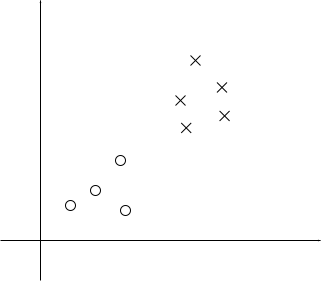
\includegraphics[width=.4\textwidth]{supervised}
    \caption{Labelled data for supervised learning\label{fig:supervised}}
  \end{center}
\end{figure}
Here are two examples for problems of different learning problems (given \emph{labelled} data as shown in Figure \ref{fig:supervised}):
\begin{itemize}
  \item Regression problem (\emph{continuous} value): estimating house price given size in square feet
  \item Classification problem (\emph{discrete} values): determine whether a tumor is malignant or benign given size of tumor and age of person
\end{itemize}

\subsection{Unsupervised Learning}
\begin{figure}[htbp]
  \begin{center}
    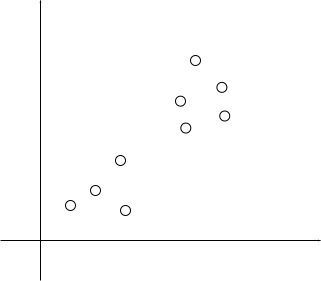
\includegraphics[width=.4\textwidth]{unsupervised}
    \caption{Data without labels\label{fig:unsupervised}}
  \end{center}
\end{figure}
When the data is not labelled (see \emph{unlabelled} data in Figure \ref{fig:unsupervised}), one can still apply clustering algorithms to it.
For example Google News clusters groups related news articles into stories.
Another basic but impressive example is separating two audio sources (speaker and a radio) using data from two microphones.

For development Andrew Ng recommends GNU Octave\citep{octave}.

\section{Linear Regression with One Variable}
\subsection{Model Representation}
\begin{table}[htbp]
  \begin{center}
    \begin{tabular}{r|r}\toprule
      \multicolumn{1}{c|}{\textbf{Size in feet$^2$ $(x)$}} &
      \multicolumn{1}{c}{\textbf{Price (\$) in 1000's $(y)$}}\\\midrule
      2104 & 460\\
      1416 & 232\\
      1534 & 315\\
       852 & 178\\
      $\vdots$ & $\vdots$\\\bottomrule
    \end{tabular}
    \caption{Table of house size and price\label{tbl:houses}}
  \end{center}
\end{table}
\newcommand{\sxi}{\ensuremath{x^{(i)}}}
\newcommand{\syi}{\ensuremath{y^{(i)}}}
\newcommand{\sumi}{\ensuremath{\displaystyle\sum_{i=1}^m}}
House price depending on house size example (see Table \ref{tbl:houses}): supervised regression problem.
The training set is denoted $(x,y)$ and the $i$th sample is $(\sxi,\syi)$ with $i\in\{1,2,\ldots,m\}$ where $m$ is the number of training samples.

The result of the learning algorithm is a \emph{hypothesis} $h$ which maps $x^\prime$ to an estimated value $y^\prime$.
\emph{E.g.} here the hypothesis is the linear function $h_\theta(x)=\theta_0+\theta_1\,x$.

Linear regression with one variable (the variable here is $x$) can also be called \emph{univariate} linear regression.

\subsection{Cost Function}
The aim is to minimize the $h_\theta(x)-y$.
\emph{I.e.} minimizing the cost function (or square error function) $J(\theta_0,\theta_1)$ in the following equation
\begin{equation*}
  \displaystyle\mathop{argmin}_{\theta_0,\theta_1}\underbrace{\frac{1}{2\,m}\,\sumi\big(h_\theta(\sxi)-\syi\big)^2}_{\eqqcolon J(\theta_0,\theta_1)}
\end{equation*}

\subsection{Cost Function Intuition}
With the simplified hypothesis $h_\theta(x)=\theta_1\,x$ we get
\begin{equation*}
  \theta_1=\mathop{argmin}_{\theta_1}J(\theta_1)=\mathop{argmin}_{\theta_1}\frac{1}{2\,m}\,\sumi\big(\theta_1\,\sxi-\syi\big)^2
\end{equation*}
The minimum can be obtained by solving for where the derivative is zero
\begin{equation*}
  \frac{\delta}{\delta\theta_1}J(\theta_1)=\frac{1}{m}\,\sumi\big(\theta_1\,\sxi-\syi\big)\,\sxi\overset{!}{=}0\Leftrightarrow
  \theta_1=\sumi\sxi\,\syi\bigg/\sumi\sxi\,\sxi
\end{equation*}
Using a contour plot one can visualise the two-dimensional version of $J(\theta_0,\theta_1)$ when using the full model.

Least-square estimation for $h_\theta(x)=\theta_0+\theta_1\,x$ yields
\begin{equation*}
\frac{1}{m}\,\sumi\big(\theta_0+\theta_1\,\sxi-\syi\big)\,\begin{pmatrix}1\\\sxi\end{pmatrix}\overset{!}{=}\vec{0}\Leftrightarrow
\begin{pmatrix}\theta_0\\\theta_1\end{pmatrix}=
\begin{pmatrix}m&\sum\sxi\\\sum\sxi&\sum\sxi\,\sxi\end{pmatrix}^{-1}\,
\begin{pmatrix}\sum\syi\\\sum\sxi\,\syi\end{pmatrix}
\end{equation*}
See Appendix \ref{app:lse} for the implementation. Figure \ref{fig:lse} shows sample data with a least square fit.
\begin{figure}[htbp]
  \begin{center}
    \includegraphics[width=.6\textwidth]{least_squares}
    \caption{Example data and corresponding least square fit of a linear function\label{fig:lse}}
  \end{center}
\end{figure}

\subsection{Gradient Descent}\label{cha:gradientdescent}
Starting from an initial solution $\theta_j$ with $j\in\{0,1\}$, the solution is updated iteratively using
\begin{equation*}
  \theta_j\coloneqq\theta_j-\alpha\,\frac{\delta}{\delta\theta_j}J(\theta_0,\theta_1)
\end{equation*}
where $\alpha$ is the learning rate.
Note that the parameters are updated ``simultaneously'' using the gradient vector $\delta J/\delta\theta$
\begin{equation}\label{equ:gradientdescent}
  \theta\coloneqq\theta-\alpha\,\frac{\delta}{\delta\theta}J(\theta)
\end{equation}

\subsection{Gradient Descent Intuition}
\begin{itemize}
  \item If $\alpha$ is too small, the algorithm will converge slowly.
  \item If $\alpha$ is too large, the algorithm will not converge on the local minimum.
\end{itemize}

\subsection{Gradient Descent for Linear Regression}
Gradient descent is performed using Equation (\ref{equ:gradientdescent}). Here the gradient is
\begin{equation*}
  \frac{\delta}{\delta\theta}J(\theta)=
  \frac{1}{m}\,\sumi\big(\theta_0+\theta_1\,\sxi-\syi\big)\,\begin{pmatrix}1\\\sxi\end{pmatrix}=
  \frac{1}{m}\,\begin{pmatrix}m&\sum\sxi\\\sum\sxi&\sum\sxi\,\sxi\end{pmatrix}\,
  \begin{pmatrix}\theta_0\\\theta_1\end{pmatrix}
\end{equation*}

See Appendix \ref{app:gradientdescent} for an implementation using symbolic differentiation of the cost function $J$.
A result of the iterative algorithm is shown in Figure \ref{fig:gradient_descent}.
\begin{figure}[htbp]
  \begin{center}
    \includegraphics[width=.6\textwidth]{gradient_descent}
    \caption{Example data and corresponding least square fit of a linear function\label{fig:gradient_descent}}
  \end{center}
\end{figure}

\section{Linear Regression with Multiple Variables}
\subsection{Multiple Features}
In the case of $n$ features, each feature $\sxi$ is a $n+1$ dimensional feature vector with $x_0$ set to $1$ for convenience:
\begin{equation*}
  \sxi=\begin{pmatrix}\sxi_0\\\sxi_1\\\vdots\\\sxi_n\end{pmatrix}\in\mathbb{R}^{n+1}
  \mathrm{\ where\ }\sxi_0\coloneqq 1
\end{equation*}
The hypothesis $h$ is
\begin{equation*}
  h_\theta(x)=\theta_0+\theta_1\,x_1+\theta_2\,x_2+\ldots+\theta_n\,x_n
\end{equation*}
Using $x_0=1$ the hypothesis can be written more compactly using the vector inner product:
\begin{equation*}
  h_\theta(x)=\theta^\top x
\end{equation*}
Regression using multiple variables is called \emph{multivariate regression}.

\subsection{Gradient Descent for Multiple Variables}
The cost function $J$ can be written using vector notation
\begin{equation*}
  J(\theta)=\frac{1}{2\,m}\sumi\big(h_\theta(\sxi)-\syi\big)^2
\end{equation*}
As in Section \ref{cha:gradientdescent}, gradient descent is performed using the parameter $\alpha$:
\begin{equation*}
  \theta_j\coloneqq\theta_j-\alpha\,\frac{\delta}{\delta\theta_j}J(\theta)\mathrm{\ for\ }j\in\{0,\ldots,n\}
\end{equation*}

\appendix
\section{Appendix}
\subsection{Least Squares Estimator}\label{app:lse}
\inputminted[frame=lines,linenos,fontsize=\small]{python}{least_squares.py}

\subsection{Gradient Descent}\label{app:gradientdescent}
\inputminted[frame=lines,linenos,fontsize=\small]{python}{gradient_descent.py}

\subsection{Convolution using Theano}
\inputminted[frame=lines,linenos,fontsize=\small]{python}{convolution.py}

\section{References}
\printbibliography[heading=none]

\end{document}
